% =====================================================================
% NaviPath / "Selection Forgetting" -- COMPAYL (MICCAI workshop) v1.0
% Self-contained LNCS document. Drop into Overleaf with:
%   - references.bib   (provided)
%   - figs/*.pdf       (copy from outputs/figs/)
% If llncs.cls / splncs04.bst are unavailable, switch \documentclass to
% {article} and the bibliography style to {plain} (see comments below).
% =====================================================================
\documentclass[runningheads]{llncs}

\usepackage{graphicx}
\usepackage{amsmath,amssymb}
\usepackage{booktabs}
\usepackage{array}
\usepackage{xcolor}
\usepackage[hidelinks]{hyperref}
\graphicspath{{figs/}{outputs/figs/}}

% ---- handy macros ----
\newcommand{\go}{\ensuremath{\checkmark}}
\newcommand{\nogo}{\ensuremath{\times}}
\newcommand{\K}{\ensuremath{K}}

\begin{document}

\title{Selection Forgetting: Continual Patch Routing Forgets Old Tasks
in Frozen-Foundation-Model Whole-Slide Image Classification}
\titlerunning{Selection Forgetting}

\author{Anonymous}
\authorrunning{Anonymous}
\institute{Anonymous Institution \\ \email{anon@anon.org}}

\maketitle

% =====================================================================
\begin{abstract}
Frozen pathology foundation models with prompt-based multiple-instance
learning make continual whole-slide image (WSI) classification attractive:
the encoder cannot drift, removing the classic source of catastrophic
forgetting. Yet under compute budgets a model must still decide \emph{which}
of a slide's thousands of patches to examine---a learnable step whose
behaviour under continual learning has not been studied. We attach a
lightweight trainable patch router to a frozen CONCH$+$QPMIL backbone and,
because the predictor never consumes router-modified features (backbone
forgetting is zero by construction), isolate the selection mechanism. On the
most-recently-learned task the router selects more informative patches than
random, prototype, and semantic heuristics ($+2.5$--$6.7$\,pp at a 64-patch
budget; 6/6 across folds and orders). On \emph{old} tasks, however, its
selection quality collapses \textbf{below random} (6/6), a phenomenon we call
\textbf{selection forgetting}. A same-task recency-flip test---varying only
whether a task was learned last vs.\ first---drops accuracy from ${\sim}0.9$ to
$0.33$--$0.40$ and holds even for the sample-abundant lung task, ruling out
difficulty/size confounds; a feature-space analysis shows the forgotten router
\emph{confidently mis-prioritizes} rather than degrading to noise. Finally,
selection forgetting is recoverable in principle---a per-task router restores
old-task selection from $0.33$ to $0.93$ (all-patch level; 3/3 folds)---but a
standard replay-free fix (EWC-on-router) does not ($0.40$; 0/3), motivating
selection-aware continual learning. We release code, configs, and figures.

\keywords{Continual learning \and Whole-slide images \and Patch selection
\and Foundation models \and Catastrophic forgetting.}
\end{abstract}

% =====================================================================
\section{Introduction}
\label{sec:intro}

Whole-slide images (WSIs) are gigapixel and are usually classified under the
multiple-instance learning (MIL) paradigm, where a slide is treated as a bag
of many patch features aggregated into a slide-level prediction
\cite{ilse2018abmil,lu2021clam}. Recent pathology foundation models supply
strong \textbf{frozen} patch encoders \cite{lu2024conch,chen2024uni}, and
prompt-based vision--language MIL adapts them to new tasks by learning only a
small set of prompts/prototypes while the encoder stays frozen
\cite{gou2025qpmil}. Freezing the encoder is attractive for continual
learning: the representation cannot drift, so the classic source of
catastrophic forgetting is largely removed. Yet a second, practical problem
remains: a slide contains thousands of patches, and under compute or latency
budgets a model must decide \textbf{which patches to look at}. This selection
step is itself learnable, and whether it survives continual learning has, to
our knowledge, not been examined.

Most continual-learning research targets forgetting of the \textbf{classifier
or representation}, and mitigates it with regularization, distillation, or
replay \cite{kirkpatrick2017ewc,li2017lwf,rebuffi2017icarl}, including
prompt-based variants for frozen backbones
\cite{wang2022l2p,wang2022dualprompt}. In contrast, the
\textbf{patch-selection / attention mechanism} that decides what the model
attends to has not been studied as a locus of forgetting. Our setting isolates
exactly this question: because the prediction backbone is frozen and never
consumes router-modified features, backbone-level forgetting is zero
\textbf{by construction}, so any degradation we observe must come from the
selection module alone.

We add a lightweight, continually-trained patch router on top of a frozen
CONCH$+$QPMIL backbone: it scores each patch and keeps the Top-\K{}, which are
then classified by the unchanged backbone. We first verified that such a
router is useful---on the \textbf{most-recently-learned} task it selects more
informative patches than random, prototype, and semantic heuristics at tight
budgets (e.g.\ $+2.5$--$6.7$\,pp at $\K{=}64$, 6/6 GO across folds and orders).
However, when we evaluate the router on \textbf{old} tasks after it has been
trained on later ones, its selection quality \textbf{collapses below the random
baseline} (6/6 NO-GO). We call this phenomenon \textbf{selection forgetting}. A
clean, single-variable test confirms the cause is recency rather than task
difficulty or sample size: for the \emph{same} task and test set, merely
changing whether it was learned \textbf{last} vs.\ \textbf{first} flips router
accuracy from ${\sim}0.9$ to $0.33$--$0.40$, and this holds even for the
sample-abundant lung task. A feature-space visualization shows the forgotten
router does not become random noise but \textbf{confidently mis-prioritizes},
selecting a patch population made salient by later tasks---explaining why it
can fall \emph{below} random.

Finally, we ask whether selection forgetting is recoverable. Storing a
separate router per task (an upper bound) \textbf{fully restores} old-task
selection (the oldest task's $\K{=}64$ accuracy returns from $0.33$ to $0.93$,
matching all-patch accuracy and beating all heuristics; 3/3 folds), proving the
signal is intact and the failure is genuine forgetting. A standard replay-free
fix---Elastic Weight Consolidation applied to the router---does \textbf{not}
suffice ($0.40$; 0/3), indicating that weight-level regularization is
inadequate for selection forgetting and that selection-aware continual methods
are needed. This question---how an autonomous selection/routing policy should
persist across tasks---connects to the emerging interest in
\emph{agentic AI for pathology} featured by this venue.

\noindent\textbf{Contributions.}
\begin{enumerate}
\item We identify and name \textbf{selection forgetting}: in
frozen-foundation-model continual WSI classification, a trainable patch router
forgets how to select patches for old tasks, even when the predictor cannot
forget.
\item We provide a \textbf{clean causal demonstration} via a same-task
recency-flip test (controlling task, data, and router; varying only recency)
and \textbf{rule out} sample-size/difficulty confounds using the
sample-abundant lung task (6/6).
\item We give a \textbf{mechanistic} account: the forgotten router
mis-prioritizes (selecting later-task-salient patches) rather than degrading to
noise, which explains sub-random behaviour.
\item We show selection forgetting is \textbf{recoverable in principle}
(per-task router upper bound) but \textbf{not fixed by EWC-on-router},
motivating selection-aware continual learning as future work.
\end{enumerate}

% =====================================================================
\section{Related Work}
\label{sec:related}

\noindent\textbf{MIL for whole-slide images.} Computational pathology
typically casts WSI classification as multiple-instance learning (MIL): a slide
is a bag of patch features pooled into a slide-level prediction
\cite{ilse2018abmil}. Attention- and transformer-based aggregators improve this
pooling \cite{lu2021clam,shao2021transmil,li2021dsmil}. These methods assume
all (or a fixed sampling of) patches are available at inference and do not study
\emph{which} patches to keep under a budget across tasks.

\noindent\textbf{Foundation models and vision--language MIL in pathology.}
Large pretrained encoders provide strong frozen patch features
\cite{chen2024uni,lu2024conch,huang2023plip}, extending image--text pretraining
\cite{radford2021clip} to histology. Prompt-based vision--language MIL keeps the
encoder frozen and learns lightweight prompts/prototypes for classification,
including continually \cite{gou2025qpmil}. We build on a frozen CONCH $+$
prompt-based QPMIL head and add a patch-selection module on top.

\noindent\textbf{Continual learning.} Methods against catastrophic forgetting
fall into regularization \cite{kirkpatrick2017ewc}, distillation
\cite{li2017lwf}, and replay
\cite{rebuffi2017icarl,chaudhry2019agem,buzzega2020der}. Prompt-based continual
learning adapts frozen backbones with small prompts
\cite{wang2022l2p,wang2022dualprompt,smith2023coda}. Crucially, this literature
studies forgetting of the \textbf{classifier/representation}; we instead expose
forgetting of a \textbf{patch-selection} mechanism and test whether a standard
replay-free regularizer (EWC, on the router) can mitigate it.

\noindent\textbf{Budget-constrained inference and patch selection.} To cut
compute, prior work selects informative patches/regions \cite{bergner2023ips}
or uses attention as saliency \cite{ilse2018abmil}. We compare a learned router
against training-free selectors (random / prototype / semantic) under explicit
budgets.

\noindent\textbf{Mixture-of-Experts / routing.} Conditional computation routes
inputs to experts \cite{shazeer2017moe,fedus2022switch}, with load-balancing to
prevent expert collapse. We borrow only the routing idea (a per-patch scalar
router) and report MoE variants as ablations.

\noindent\textbf{Gap.} To our knowledge, no prior work studies whether a
\emph{trainable patch selector} itself forgets across tasks in frozen-FM
continual WSI classification. We name and quantify this \textbf{selection
forgetting}, give a clean same-task recency-flip causal test, and show it is
recoverable in principle (per-task upper bound) yet not fixed by weight-level
consolidation.

% =====================================================================
\section{Method}
\label{sec:method}

\noindent\textbf{Notation.} A slide has $n$ patches with frozen CONCH features
$z_i\in\mathbb{R}^{512}$; $\hat{(\cdot)}$ denotes L2-normalization,
$\{t_c\}_{c=1}^{C}$ class-text features, $\{p_m\}_{m=1}^{M}$ prototype features,
and $\phi$ the router parameters.

\subsection{Problem setup}
We study class-incremental WSI classification under a fixed feature budget.
Tasks $t=1,\dots,T$ arrive sequentially; after task $t$ the model classifies
slides from all seen tasks using at most \K{} patches per slide ($\K\ll n$). We
separate two sub-problems usually conflated: \emph{what to predict}
(classifier) and \emph{what to look at} (selection).

\subsection{Decoupled prediction backbone}
Prediction reuses a prompt-based continual MIL head (QPMIL) on the frozen CONCH
features. The prediction path never consumes router- or expert-transformed
features:
\begin{equation}
\hat{y} = \arg\max\; g_{\theta^\ast}\!\big(\{z_i\}_{i\in\mathcal{S}}\big),
\qquad \theta^\ast \text{ frozen}\;\Rightarrow\;
\mathrm{Forgetting}\equiv 0 .
\label{eq:decouple}
\end{equation}
Hence backbone-level forgetting is zero \textbf{by construction}
(Fig.~\ref{fig:rmatrix}), an identity we report transparently rather than as a
contribution.

\subsection{Trainable patch router}
For each patch we compute four task-count-invariant summary statistics (max and
entropy of class-text similarity; max and mean prototype similarity) and map
$[z_i;s_i]$ through a two-layer MLP to a scalar importance $r_i$:
\begin{equation}
s_i = \Big[\max_c \hat{z}_i^\top \hat{t}_c,\;
           H(\mathrm{softmax}_c\,\hat{z}_i^\top \hat{t}),\;
           \max_m \hat{z}_i^\top \hat{p}_m,\;
           \tfrac{1}{M}\textstyle\sum_m \hat{z}_i^\top \hat{p}_m\Big],
\qquad r_i = \mathrm{MLP}_\phi([z_i;s_i]).
\label{eq:score}
\end{equation}
At inference we keep the Top-\K{} patches:
\begin{equation}
\mathcal{S}_K = \underset{i}{\mathrm{top\text{-}}K}\; r_i,
\qquad |\mathcal{S}_K|=K.
\label{eq:topk}
\end{equation}
The router ($\approx$132K params) is the only component trained across tasks;
the backbone stays frozen.

\subsection{Differentiable training}
Because hard Top-\K{} is non-differentiable, we train with a soft-route
objective: scores over the selected set are softmax-normalized into weights,
aggregated into a bag embedding, and classified by the frozen text head;
gradients reach $\phi$ only through the weights.
\begin{equation}
w_i=\frac{\exp(r_i)}{\sum_{j\in\mathcal{S}_K}\exp(r_j)},\quad
\bar{z}=\widehat{\textstyle\sum_{i\in\mathcal{S}_K} w_i z_i},\quad
\mathcal{L}_{\text{route}}=\mathrm{CE}\big(\sigma\,\bar{z}F_{\text{txt}}^\top,\,y\big).
\label{eq:softroute}
\end{equation}

\subsection{Selection baselines}
We compare the router against three training-free selectors that pick the
Top-\K{} patches by (i) random; (ii) prototype similarity
$\max_m \hat z_i^\top\hat p_m$; (iii) semantic similarity
$\max_c \hat z_i^\top\hat t_c$. All feed the same frozen backbone, so any
accuracy gap is due to selection alone (Fig.~\ref{fig:protocol}).

\subsection{Router consolidation (mitigation)}
To test recoverability we add replay-free consolidation on the router: after
each task we estimate a diagonal Fisher and penalize drift of important weights
on later tasks (EWC-on-router); we also report a \textbf{per-task router} (one
stored per task) as an empirical upper bound.
\begin{equation}
F^{(t)}_j=\mathbb{E}_{\mathcal{D}_t}\!\big[(\partial \mathcal{L}_{\text{route}}/\partial \phi_j)^2\big],\quad
\mathcal{L}^{(t+1)}=\mathcal{L}_{\text{route}}
+\lambda\!\sum_{\tau\le t}\!\sum_j F^{(\tau)}_j(\phi_j-\phi^{\ast(\tau)}_j)^2.
\label{eq:ewc}
\end{equation}

\subsection{Evaluation protocol}
Four TCGA tasks, two orders (paper/reverse), three folds, budgets
$\K\in\{\text{All},256,128,64,32\}$. We report Top-1 accuracy and a GO/NO-GO
criterion (router beats the best heuristic at a finite budget), evaluating both
the most-recent task and each old task to expose recency-dependent selection
forgetting (Fig.~\ref{fig:recency}).

\begin{figure}[t]
\centering
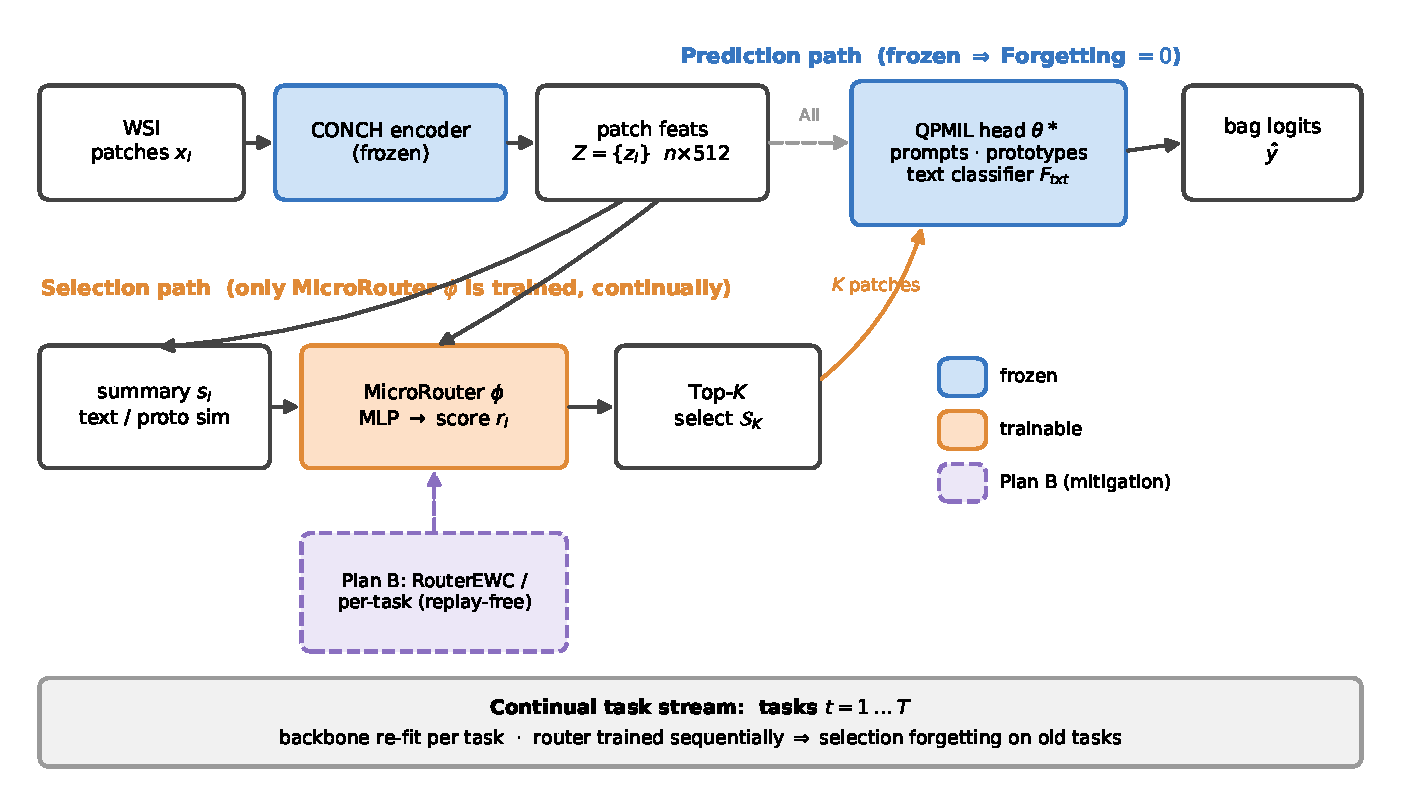
\includegraphics[width=\linewidth]{Fig1_arch.pdf}
\caption{NaviPath's decoupled design. A frozen CONCH $+$ QPMIL prediction path
(blue) shares patch features with a lightweight, continually-trained patch
router (orange) that scores patches and keeps the Top-\K{}; the selected patches
are classified by the unchanged backbone. Because the predictor never consumes
router-modified features, backbone forgetting is zero by construction, so the
router is the sole locus of continual learning. Plan B (purple, dashed)
consolidates the router (per-task / EWC).}
\label{fig:arch}
\end{figure}

% =====================================================================
\section{Experiments and Results}
\label{sec:exp}

\subsection{Experimental setup}
\textbf{Data and tasks.} We use four TCGA cohorts as a class-incremental
sequence of binary subtyping tasks---lung (NSCLC), breast (BRCA), renal (RCC),
and esophageal (ESCA)---each contributing two subtypes, for eight classes in
total (label shifts $0,2,4,6$). Patches are encoded once by a frozen CONCH
foundation model into 512-d features \cite{lu2024conch}; the encoder is never
updated. We evaluate two task orders, \textbf{paper} (lung$\to$brca$\to$rcc$\to$esca)
and \textbf{reverse} (esca$\to$rcc$\to$brca$\to$lung), each over \textbf{3 folds}
(official train/val/test splits), and report the mean. The reverse order makes
the small-sample esca the \emph{oldest} task and the large-sample lung the
\emph{most-recent}, and vice-versa for paper---enabling the same-task recency
comparison of Sec.~\ref{sec:recency}.

\noindent\textbf{Backbone (prediction path).} We adopt a prompt-based
vision--language MIL head (QPMIL) on the frozen CONCH features
\cite{gou2025qpmil}, trained per task with Adam (lr $1\mathrm{e}{-3}$, weight
decay $5\mathrm{e}{-4}$, 12 epochs/task). The same optimizer/epoch budget is
used for the QPMIL baseline and our setup, so backbone-accuracy comparisons
(Table~\ref{tab:acc}) are matched.

\noindent\textbf{Router (selection path).} The MicroRouter is a two-layer MLP
($\approx$132K parameters) mapping each patch's feature concatenated with four
task-count-invariant summary statistics to a scalar score; it is trained
continually with Adam (lr $5\mathrm{e}{-4}$, weight decay $1\mathrm{e}{-4}$, 5
epochs/task) using the differentiable soft-route objective
(Sec.~\ref{sec:method}), with the backbone frozen throughout.

\noindent\textbf{Budgets and selectors.} At inference we keep the Top-\K{}
patches for $\K\in\{\text{All},256,128,64,32\}$ and feed them to the frozen
head. We compare the learned router against three training-free selectors:
\textbf{random}, \textbf{prototype} (max cosine similarity to the QPMIL
prototype pool), and \textbf{semantic} (max cosine similarity to class-text
features). All selectors feed the identical backbone, so accuracy differences
reflect selection only (Fig.~\ref{fig:protocol}).

\noindent\textbf{GO/NO-GO criterion.} For a given task and budget we say the
router is \textbf{GO} if it exceeds the best of the three heuristics at $\K{=}64$
(router@64 $>\max\{$random, prototype, semantic$\}$@64), and \textbf{NO-GO}
otherwise. We additionally report full budget curves. (Note: esca has a small
test set, motivating the lung-based confound check in Sec.~\ref{sec:recency}.)

\subsection{Backbone accuracy and the necessity of decoupling}
Under matched training (12 epochs/task, Adam lr=1e-3, wd=5e-4) our
frozen-backbone setup attains continual accuracy on par with the QPMIL baseline
(Table~\ref{tab:acc}): QPMIL reaches ACC $0.924/0.917$ (paper/reverse) with mild
forgetting ($0.017/0.041$), while the decoupled NaviPath reaches $0.879/0.886$
with \textbf{Forgetting $=0$}. We stress that this zero is an \textbf{identity,
not a contribution}: because the prediction path is a frozen backbone that never
consumes router- or expert-modified features, per-task accuracy is flat by
construction (Fig.~\ref{fig:rmatrix}). Decoupling is \emph{necessary}: an
earlier non-decoupled variant, in which trainable experts transformed the
features fed back to the frozen backbone, induced severe interference: accuracy
collapsed to $0.378/0.218$ and forgetting rose to $0.735/0.950$ (paper/reverse),
far worse than the QPMIL baseline. We therefore fix the predictor and study the
only component that learns continually---the patch router.

\subsection{The router helps on recently-learned tasks}
On the \textbf{most-recently-learned} task, the learned router selects more
informative patches than all training-free heuristics at tight budgets
(Fig.~\ref{fig:recent}, Table~\ref{tab:router}). At $\K{=}64$ it reaches $0.956$
(esca, recent) and $0.922$ (lung, recent), versus the best heuristic $0.889$ and
$0.897$ respectively, i.e.\ $+2.5$--$6.7$\,pp; using only 64 of thousands of
patches nearly matches all-patch accuracy. This holds for both ``recent'' tasks
across all folds and orders (6/6 GO), establishing that the router \emph{can}
learn a useful, budget-efficient selection policy.

\subsection{Selection forgetting on old tasks}
The picture reverses for \textbf{old} tasks---those learned early and then
followed by other tasks. Here the router's selection quality drops \textbf{below
the random baseline} at tight budgets (Fig.~\ref{fig:old},
Table~\ref{tab:router}): $\K{=}64$ accuracy falls to $0.333$ (esca, old) and
$0.397$ (lung, old), against best heuristics of $0.822$ and $0.813$ (6/6
NO-GO). Because the predictor is unchanged, this degradation is attributable to
the selection module alone. We term this \textbf{selection forgetting}: the
router forgets how to choose patches for tasks it learned earlier.

\subsection{Same-task recency flip: a clean causal test}
\label{sec:recency}
To rule out that old tasks are simply harder or smaller, we compare the
\emph{identical} task and test set under the two orders, changing only whether
the task was learned \textbf{last} (recent) or \textbf{first} (old). Selection
accuracy flips sharply (Fig.~\ref{fig:recency}): lung $0.922\to0.397$ and esca
$0.956\to0.333$ at $\K{=}64$. Holding task, data, and router architecture fixed
and varying only recency isolates recency as the cause. Critically, the flip
also occurs for \textbf{lung}, the most sample-abundant task, excluding
sample-size/difficulty confounds. The effect replicates across all folds (6/6).

\subsection{Mechanism: confident mis-prioritization, not noise}
A shared-embedding feature-space visualization (Fig.~\ref{fig:mechanism}) scores
the \emph{same} esca slide with the router that learned esca recently vs.\ the
router that learned it long ago. The forgotten router does \textbf{not} collapse
to uniform/noisy scores; it still produces structured scores but concentrates
its Top-\K{} on a \emph{different} patch sub-population---one made salient by the
later tasks. This \textbf{confident mis-prioritization} explains why old-task
selection can fall \emph{below} random (actively wrong) rather than merely
matching it (no signal).

\subsection{Mitigation: recoverable in principle, but not by EWC}
\label{sec:mitigation}
Finally, we test recovery on the oldest task (Table~\ref{tab:planb}, 3-fold).
Storing a \textbf{separate router per task} (an empirical upper bound)
\textbf{fully restores} old-task selection: $\K{=}64$ accuracy rises from
$0.333$ to $\mathbf{0.933}$---flat across all budgets (matching all-patch
accuracy) and above every heuristic (GO 3/3). This proves the selection signal
remains intact and the failure is genuine forgetting. In contrast, a standard
replay-free regularizer, \textbf{EWC-on-router}, barely helps
($0.333\to0.400$ at $\K{=}64$, still below the $0.822$ best heuristic; NO-GO
0/3), while leaving recent-task selection unharmed (e.g.\ reverse-lung remains
GO). Weight-level consolidation is thus insufficient for selection forgetting,
motivating selection-aware approaches (Sec.~\ref{sec:discussion}).

% ---------------- Tables ----------------
\begin{table}[t]
\centering
\caption{Continual accuracy (backbone level, mean$\pm$std over 3 folds). QPMIL
baseline and NaviPath use matched training (12 epochs/task, Adam lr 1e-3,
wd 5e-4). NaviPath's Forgetting$=0$ is a decoupling identity
(Fig.~\ref{fig:rmatrix}), not a contribution; QPMIL ACC $\ge$ NaviPath, so our
contribution is the selection analysis, not ACC.}
\label{tab:acc}
\begin{tabular}{llccc}
\toprule
Method & Order & ACC & Forgetting & BWT \\
\midrule
QPMIL baseline       & paper   & $0.924\pm0.016$ & $0.017\pm0.022$ & $-0.017\pm0.022$ \\
QPMIL baseline       & reverse & $0.917\pm0.026$ & $0.041\pm0.023$ & $-0.041\pm0.023$ \\
NaviPath (decoupled) & paper   & $0.879\pm0.030$ & $0.000$         & $0.000$ \\
NaviPath (decoupled) & reverse & $0.886\pm0.030$ & $0.000$         & $0.000$ \\
\bottomrule
\end{tabular}
\end{table}

\begin{table}[t]
\centering
\caption{Router patch selection, recent vs.\ old (router accuracy at budget
\K{}, mean over 3 folds). ``best heur''$=\max\{$random, prototype, semantic$\}$;
GO if router@64 $>$ best heur@64. The router is GO on both recent tasks (6/6)
and NO-GO on both old tasks (6/6).}
\label{tab:router}
\begin{tabular}{llccccccc}
\toprule
Task & Recency & @256 & @128 & @64 & @32 & best heur@64 & GO \\
\midrule
esca & RECENT (paper, last)   & 0.956 & 0.956 & \textbf{0.956} & 0.933 & 0.889 & \go\,(3/3) \\
esca & OLD (reverse, first)   & 0.511 & 0.400 & \textbf{0.333} & 0.333 & 0.822 & \nogo\,(0/3) \\
lung & RECENT (reverse, last) & 0.904 & 0.915 & \textbf{0.922} & 0.918 & 0.897 & \go\,(3/3) \\
lung & OLD (paper, first)     & 0.512 & 0.453 & \textbf{0.397} & 0.353 & 0.813 & \nogo\,(0/3) \\
\bottomrule
\end{tabular}
\end{table}

\begin{table}[t]
\centering
\caption{Mitigation on the oldest task (esca, reverse order; router accuracy at
budget \K{}, mean over 3 folds). The per-task router (upper bound) fully
restores old-task selection to recent-task levels (GO 3/3), whereas
EWC-on-router barely moves the needle (NO-GO 0/3): weight-level consolidation is
insufficient for selection forgetting.}
\label{tab:planb}
\begin{tabular}{lcccccc}
\toprule
Router consolidation & @256 & @128 & @64 & @32 & best heur@64 & GO \\
\midrule
none (continual)            & 0.511 & 0.400 & \textbf{0.333} & 0.333 & 0.822 & \nogo\,(0/3) \\
EWC-on-router (replay-free)  & 0.622 & 0.422 & \textbf{0.400} & 0.267 & 0.822 & \nogo\,(0/3) \\
per-task router (upper bound)& 0.933 & 0.933 & \textbf{0.933} & 0.933 & 0.822 & \go\,(3/3) \\
\bottomrule
\end{tabular}
\end{table}

% ---------------- Figures ----------------
\begin{figure}[t]
\centering

\includegraphics[width=0.9\linewidth]{P0_router_v0.pdf}
\caption{Patch-budget accuracy on the most-recently-learned task. The learned
router matches or exceeds random, prototype, and semantic selectors across
budgets, with $+2.5$--$6.7$\,pp at $\K{=}64$ (6/6 GO across folds and orders);
64 of thousands of patches nearly match all-patch accuracy.}
\label{fig:recent}
\end{figure}

\begin{figure}[t]
\centering

\includegraphics[width=0.9\linewidth]{P0_oldtask_budget.pdf}
\caption{Patch-budget accuracy on an old task (learned first, then overwritten).
The router falls below random at tight budgets (router@64 $<$ random@64; 6/6
NO-GO), i.e.\ selection forgetting; training-free heuristics are unaffected.}
\label{fig:old}
\end{figure}

\begin{figure}[t]
\centering

\includegraphics[width=0.95\linewidth]{P0b_recency_flip.pdf}
\caption{\textbf{Same-task recency flip (core result).} For the identical task
and test set, the router selects well when the task was learned last
(solid, ${\sim}0.9$) but collapses below random when the same task was learned
first and overwritten (dashed, $0.33$--$0.40$). Holds for both lung and esca,
excluding sample-size/difficulty confounds.}
\label{fig:recency}
\end{figure}

\begin{figure}[t]
\centering
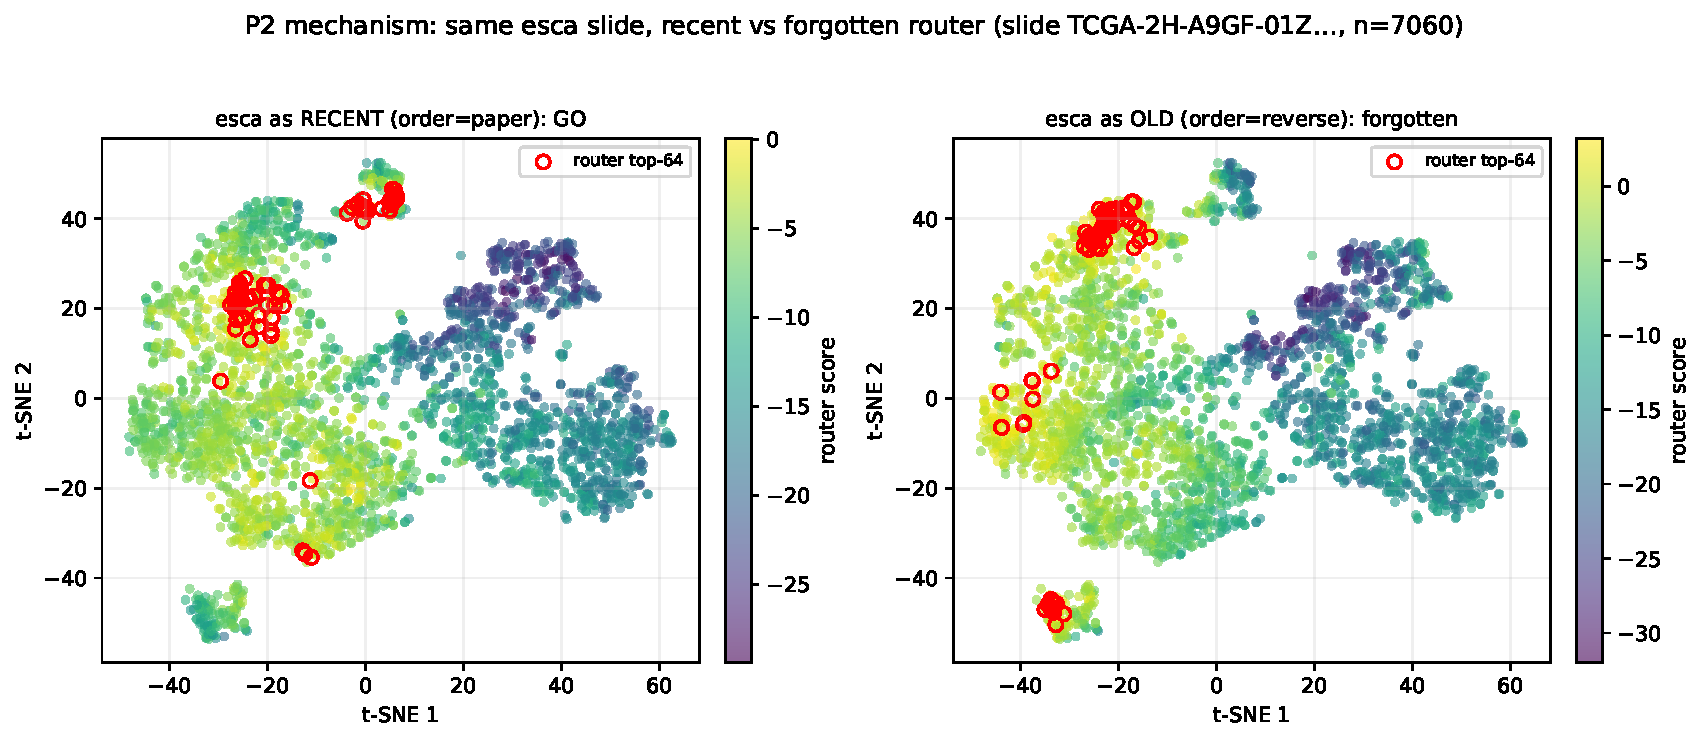
\includegraphics[width=\linewidth]{P2contrast_esca_fold1.pdf}
\caption{\textbf{Mechanism.} The same esca slide in CONCH feature space (shared
t-SNE), scored by the router when esca was recent (left) vs.\ old/overwritten
(right). The forgotten router keeps structured scores but concentrates its
Top-\K{} on a different, later-task-salient sub-population---confident
mis-prioritization, explaining sub-random behaviour.}
\label{fig:mechanism}
\end{figure}

\begin{figure}[t]
\centering

\includegraphics[width=0.85\linewidth]{P1_r_matrix.pdf}
\caption{Per-task accuracy $R[i,j]$ (accuracy on task $j$ after learning task
$i$). NaviPath columns are flat by construction (decoupled frozen backbone
$\Rightarrow$ Forgetting$=0$ is an identity), while the QPMIL baseline shows mild
genuine drift; we surface this to locate our contribution in the selection
analysis.}
\label{fig:rmatrix}
\end{figure}

\begin{figure}[t]
\centering

\includegraphics[width=\linewidth]{FigS1_arch.pdf}
\caption{\textbf{Evaluation protocol (appendix).} The router and three
training-free selectors each pick a Top-\K{} subset from the same frozen features
and feed the same frozen head; we report accuracy at budget \K{} and a GO/NO-GO
criterion. Only the selected set differs, so accuracy gaps reflect selection
alone.}
\label{fig:protocol}
\end{figure}

% =====================================================================
\section{Discussion and Limitations}
\label{sec:discussion}

\noindent\textbf{Selection forgetting is distinct from classifier forgetting.}
Our setup deliberately removes representation/classifier drift (the backbone is
frozen, so Forgetting$=0$ by construction), which lets us attribute every
old-task degradation to the selection module. The result is a forgetting
phenomenon that the continual-learning literature, focused on
classifier/representation, does not capture: even when \emph{what to predict}
cannot be forgotten, \emph{what to look at} can. We believe this matters broadly
for budget-constrained inference with frozen foundation models, where a learned
gate/router/selector sits in front of a fixed predictor.

\noindent\textbf{Why does EWC fail while a per-task router fully recovers?} The
per-task upper bound restoring old-task accuracy to the all-patch level
($0.33\to0.93$) shows the information needed to select well is still present in
the frozen features; the single continual router simply overwrites the
\emph{ranking} it had learned for old tasks. EWC penalizes drift of individual
router weights, but the quantity that matters here is the induced \emph{ordering}
of patch scores, a global, highly nonlinear function of those weights.
Protecting individual weights is therefore a poor proxy for protecting a
selection policy---suggesting that selection-aware objectives (e.g.\ distilling
old-task score rankings, or function-space/rank-preserving regularization) are a
more promising direction than weight-space penalties.

\noindent\textbf{On the honesty of Forgetting$=0$.} We report this as an
identity, not a contribution (Fig.~\ref{fig:rmatrix}), precisely to avoid
over-claiming: the decoupled design buys zero backbone forgetting at the cost of
the experts/router contributing nothing to the main accuracy metric. Our
contribution is the analysis of the selection path, not a new state-of-the-art
accuracy.

\noindent\textbf{Limitations.} (i) We study four TCGA cohorts from a single
source; broader datasets and longer task sequences would strengthen generality.
(ii) The oldest task in the reverse order (esca) has a small test set; we
mitigate this with the sample-abundant lung task, which shows the same recency
flip, but larger cohorts remain desirable. (iii) The router is a scalar v0;
richer selectors (set-level or attention-based) may exhibit different dynamics.
(iv) Our mitigation study (Table~\ref{tab:planb}) is demonstrated on the oldest
task over all 3 folds; extending the per-task/EWC comparison to every task and
order is left as future work, though the upper-bound recovery and EWC
insufficiency are highly consistent across folds (3/3).

% =====================================================================
\section{Conclusion}
\label{sec:conclusion}
We show that adding a trainable patch router to a frozen-foundation-model
continual WSI classifier introduces \textbf{selection forgetting}: the router
selects well for the most-recent task but, for older tasks, falls below a random
baseline. A same-task recency-flip test establishes recency as the cause and
excludes sample-size confounds, and a feature-space analysis reveals confident
mis-prioritization rather than noise. The phenomenon is recoverable in
principle---a per-task router restores old-task selection to the all-patch
level---yet a standard replay-free regularizer (EWC-on-router) does not fix it.
We argue that \textbf{selection-aware continual learning} is needed when a
learned selector front-ends a frozen predictor, and we release our code,
configs, and figures to support follow-up work.

% =====================================================================
% Bibliography. For LNCS use splncs04; if unavailable switch to {plain}.
\bibliographystyle{splncs04}
\bibliography{references}

\end{document}
